% Options for packages loaded elsewhere
\PassOptionsToPackage{unicode}{hyperref}
\PassOptionsToPackage{hyphens}{url}
%
\documentclass[
]{article}
\usepackage{amsmath,amssymb}
\usepackage{iftex}
\ifPDFTeX
  \usepackage[T1]{fontenc}
  \usepackage[utf8]{inputenc}
  \usepackage{textcomp} % provide euro and other symbols
\else % if luatex or xetex
  \usepackage{unicode-math} % this also loads fontspec
  \defaultfontfeatures{Scale=MatchLowercase}
  \defaultfontfeatures[\rmfamily]{Ligatures=TeX,Scale=1}
\fi
\usepackage{lmodern}
\ifPDFTeX\else
  % xetex/luatex font selection
\fi
% Use upquote if available, for straight quotes in verbatim environments
\IfFileExists{upquote.sty}{\usepackage{upquote}}{}
\IfFileExists{microtype.sty}{% use microtype if available
  \usepackage[]{microtype}
  \UseMicrotypeSet[protrusion]{basicmath} % disable protrusion for tt fonts
}{}
\makeatletter
\@ifundefined{KOMAClassName}{% if non-KOMA class
  \IfFileExists{parskip.sty}{%
    \usepackage{parskip}
  }{% else
    \setlength{\parindent}{0pt}
    \setlength{\parskip}{6pt plus 2pt minus 1pt}}
}{% if KOMA class
  \KOMAoptions{parskip=half}}
\makeatother
\usepackage{xcolor}
\usepackage[margin=1in]{geometry}
\usepackage{longtable,booktabs,array}
\usepackage{calc} % for calculating minipage widths
% Correct order of tables after \paragraph or \subparagraph
\usepackage{etoolbox}
\makeatletter
\patchcmd\longtable{\par}{\if@noskipsec\mbox{}\fi\par}{}{}
\makeatother
% Allow footnotes in longtable head/foot
\IfFileExists{footnotehyper.sty}{\usepackage{footnotehyper}}{\usepackage{footnote}}
\makesavenoteenv{longtable}
\usepackage{graphicx}
\makeatletter
\def\maxwidth{\ifdim\Gin@nat@width>\linewidth\linewidth\else\Gin@nat@width\fi}
\def\maxheight{\ifdim\Gin@nat@height>\textheight\textheight\else\Gin@nat@height\fi}
\makeatother
% Scale images if necessary, so that they will not overflow the page
% margins by default, and it is still possible to overwrite the defaults
% using explicit options in \includegraphics[width, height, ...]{}
\setkeys{Gin}{width=\maxwidth,height=\maxheight,keepaspectratio}
% Set default figure placement to htbp
\makeatletter
\def\fps@figure{htbp}
\makeatother
\setlength{\emergencystretch}{3em} % prevent overfull lines
\providecommand{\tightlist}{%
  \setlength{\itemsep}{0pt}\setlength{\parskip}{0pt}}
\setcounter{secnumdepth}{5}
\usepackage{float}
\usepackage{multirow}
\usepackage{lastpage}
\usepackage{fancyhdr}
\pagestyle{fancy}
\usepackage{booktabs}
\usepackage{longtable}
\usepackage{array}
\usepackage{multirow}
\usepackage{wrapfig}
\usepackage{float}
\usepackage{colortbl}
\usepackage{pdflscape}
\usepackage{tabu}
\usepackage{threeparttable}
\usepackage{threeparttablex}
\usepackage[normalem]{ulem}
\usepackage{makecell}
\usepackage{xcolor}
\ifLuaTeX
  \usepackage{selnolig}  % disable illegal ligatures
\fi
\IfFileExists{bookmark.sty}{\usepackage{bookmark}}{\usepackage{hyperref}}
\IfFileExists{xurl.sty}{\usepackage{xurl}}{} % add URL line breaks if available
\urlstyle{same}
\hypersetup{
  pdftitle={HCD Simulations Write Up},
  pdfauthor={Audrey Fu Lab},
  hidelinks,
  pdfcreator={LaTeX via pandoc}}

\title{HCD Simulations Write Up}
\author{Audrey Fu Lab}
\date{2024-03-07}

\begin{document}
\maketitle

\section*{Simulation Description}

\section*{Preliminary Findings}

\newpage
\section*{Figures}

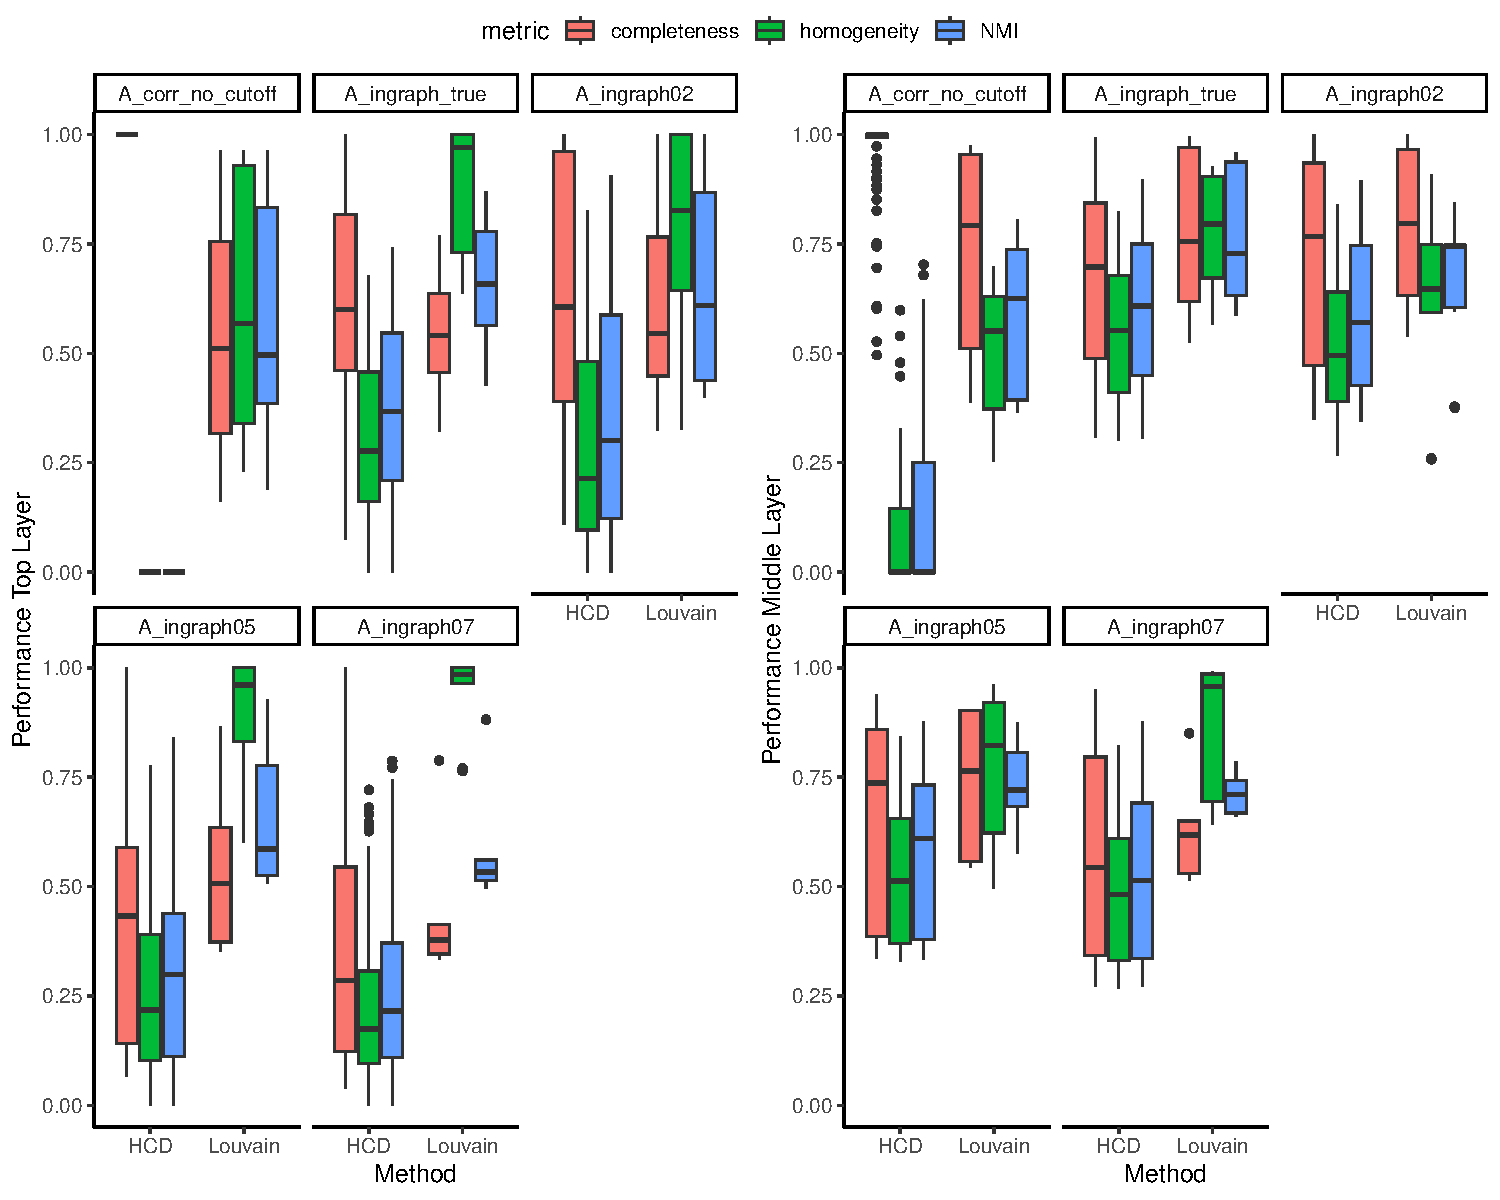
\includegraphics{Lab_report_3_13_2024_files/figure-latex/unnamed-chunk-1-1.pdf}

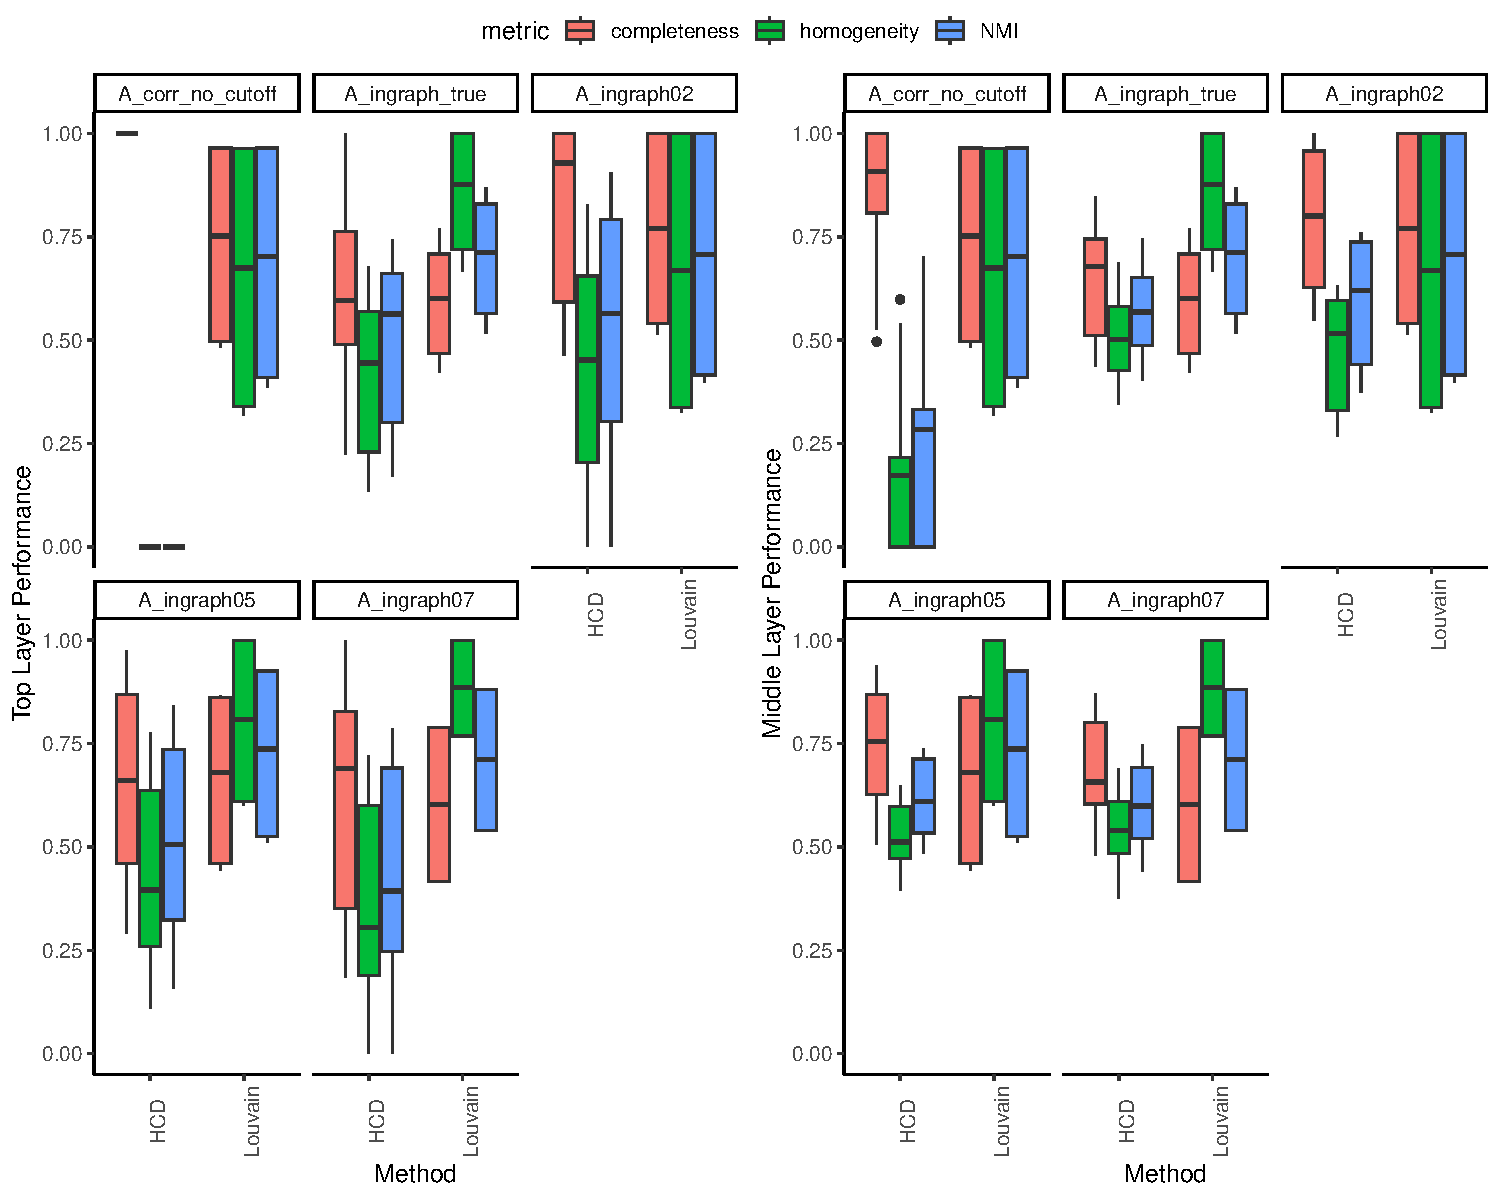
\includegraphics{Lab_report_3_13_2024_files/figure-latex/unnamed-chunk-2-1.pdf}

\begin{figure}
\centering
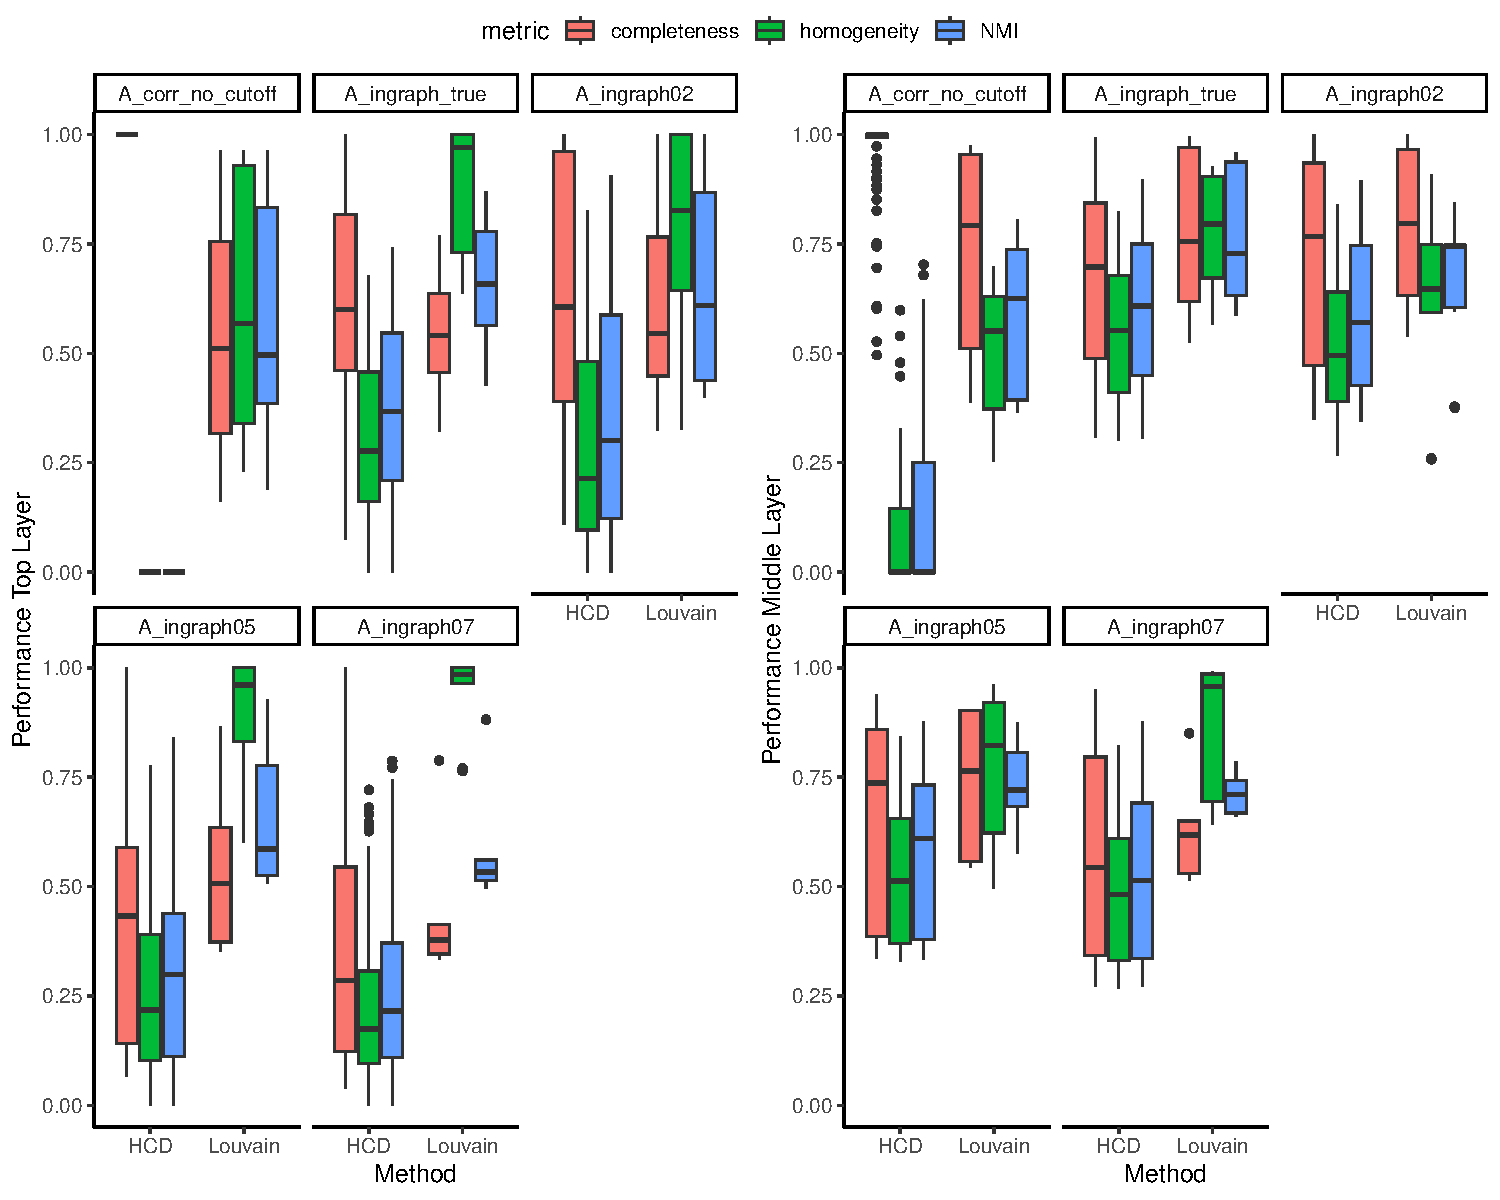
\includegraphics{Lab_report_3_13_2024_files/figure-latex/unnamed-chunk-3-1.pdf}
\caption{Small world graphs}
\end{figure}

\begin{figure}
\centering
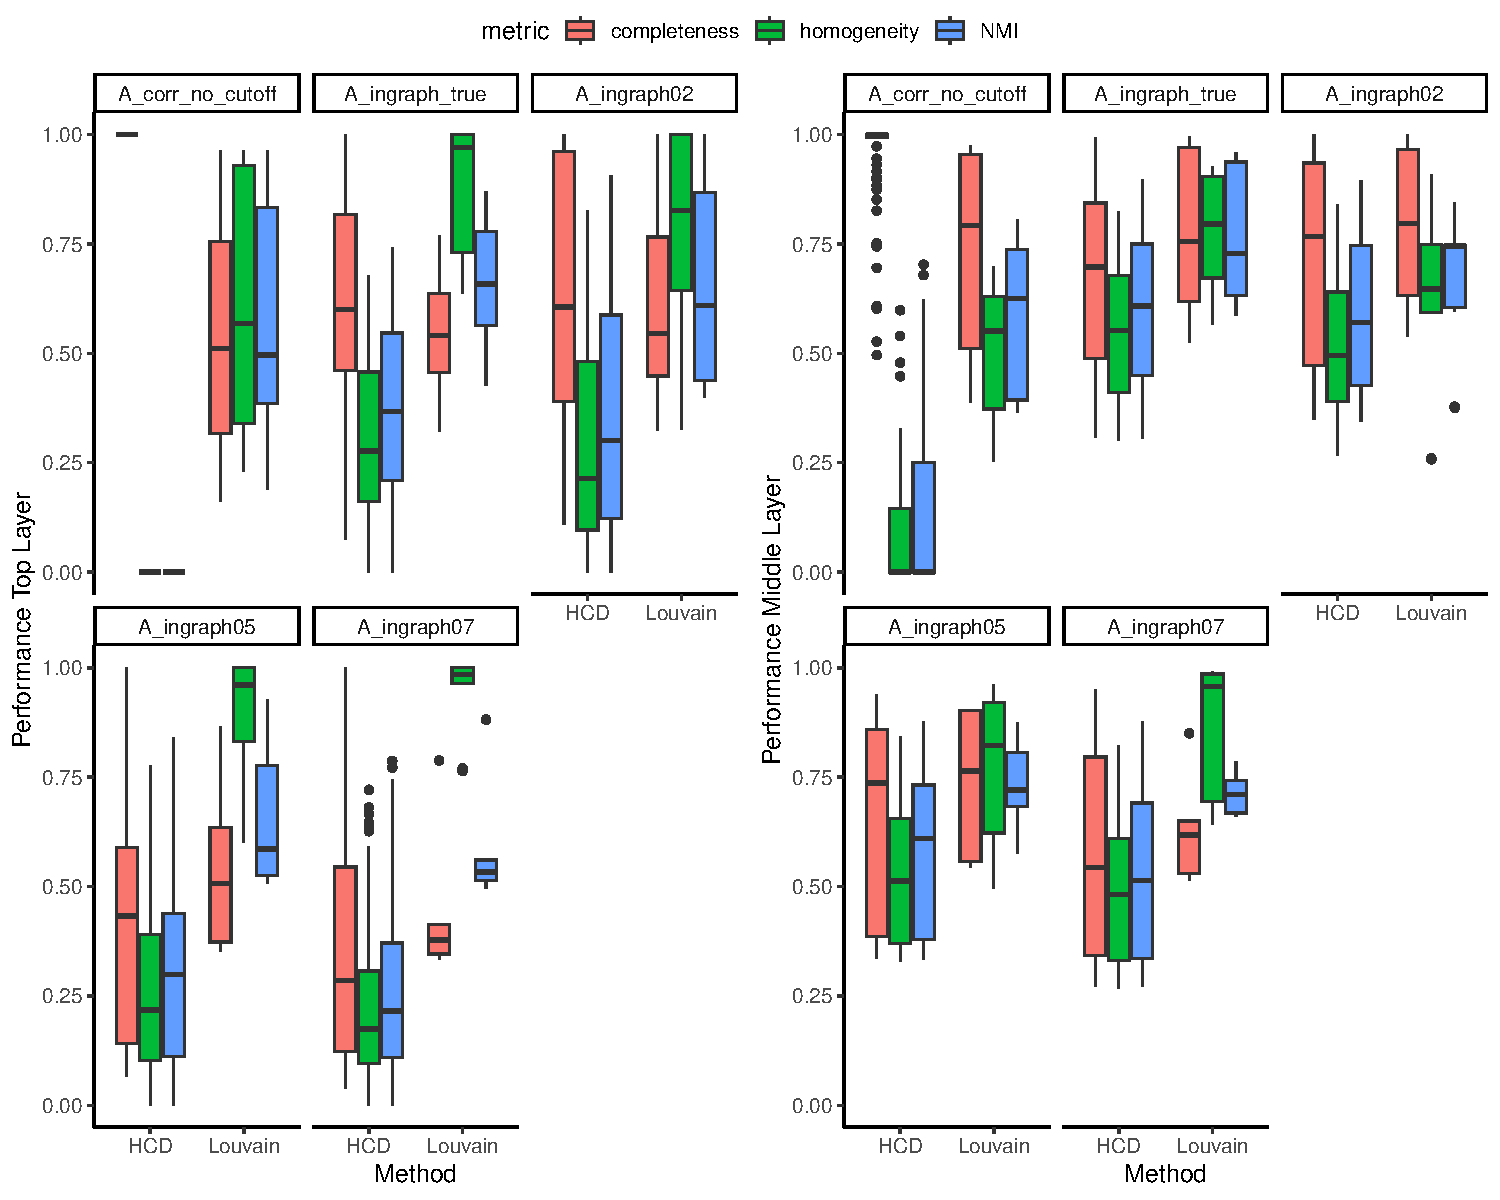
\includegraphics{Lab_report_3_13_2024_files/figure-latex/unnamed-chunk-4-1.pdf}
\caption{Scale free graphs}
\end{figure}

\begin{figure}
\centering
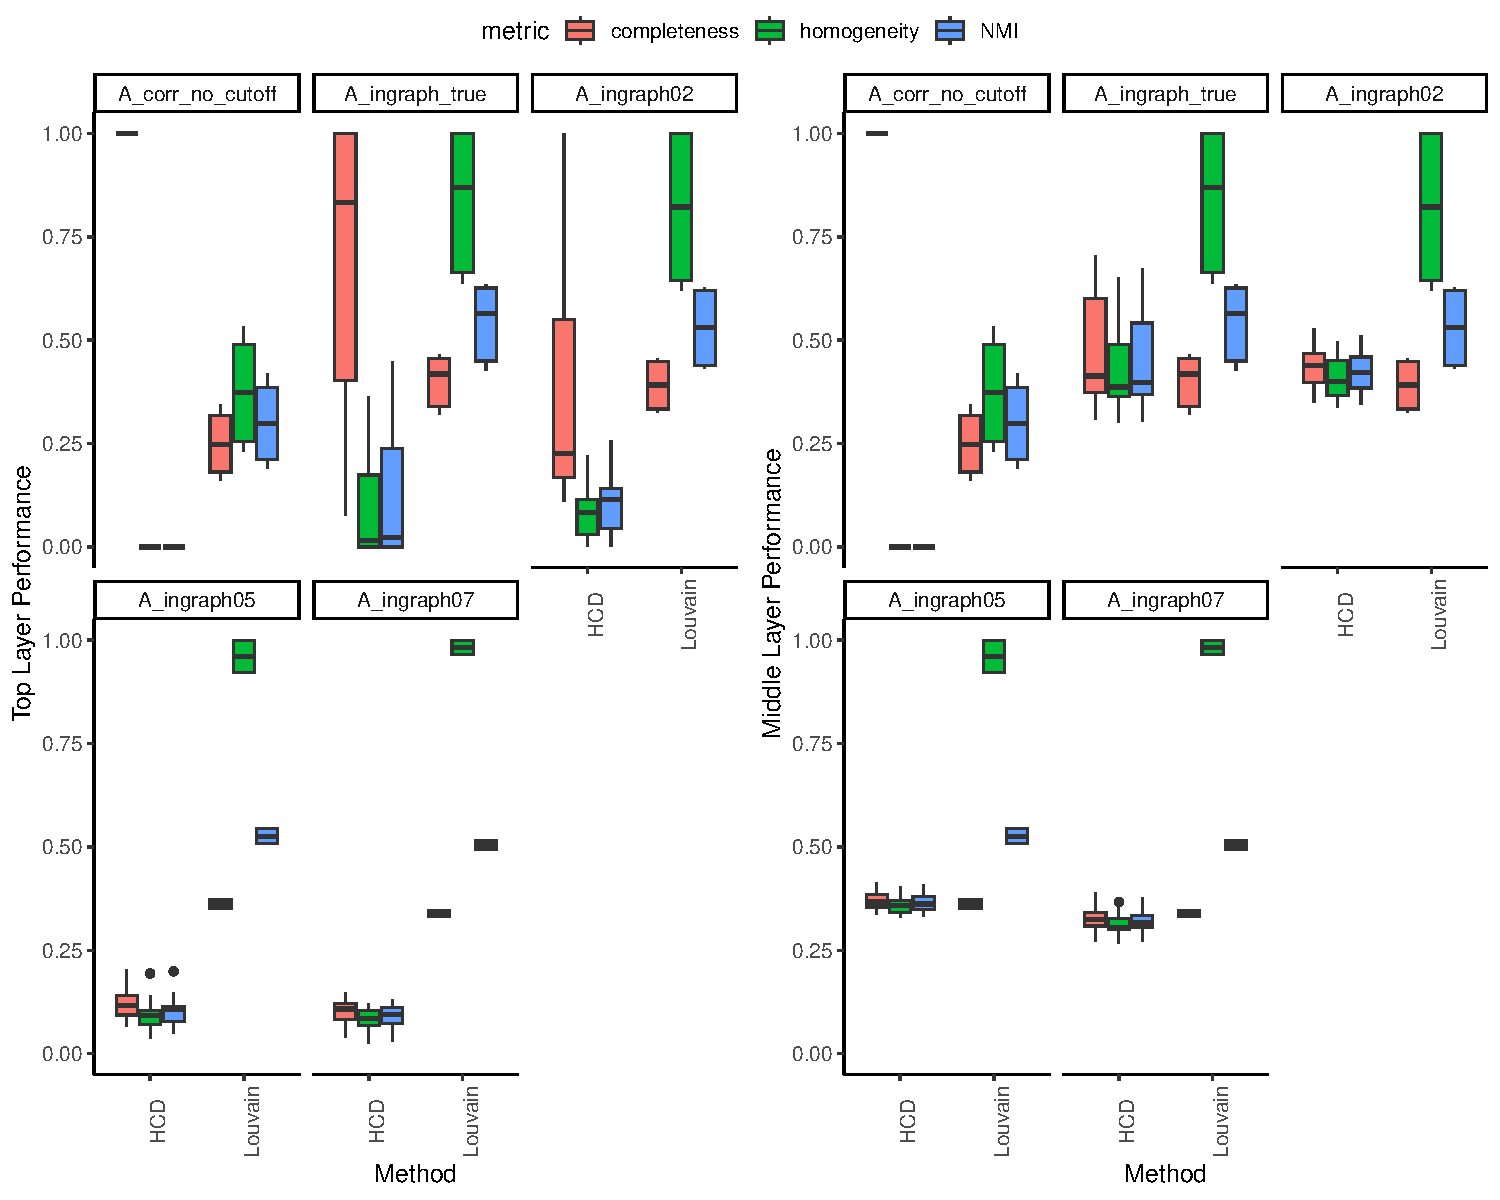
\includegraphics{Lab_report_3_13_2024_files/figure-latex/unnamed-chunk-5-1.pdf}
\caption{random graphs}
\end{figure}

\newpage 
\section*{Tables}

\begin{table}

\caption{\label{tab:unnamed-chunk-6}Summary statistics for intermediate difficulty simulated networks.}
\centering
\fontsize{10}{12}\selectfont
\fontsize{10}{12}\selectfont
\begin{tabular}[t]{>{\raggedright\arraybackslash}p{8em}llllll}
\toprule
Value & Network1 & Network2 & Network3 & Network4 & Network5 & Network6\\
\midrule
\cellcolor{gray!6}{Subgraph type} & \cellcolor{gray!6}{small world} & \cellcolor{gray!6}{small world} & \cellcolor{gray!6}{scale free} & \cellcolor{gray!6}{scale free} & \cellcolor{gray!6}{random graph} & \cellcolor{gray!6}{random graph}\\
Connection type & disc & full & disc & full & disc & full\\
\cellcolor{gray!6}{Layers} & \cellcolor{gray!6}{3} & \cellcolor{gray!6}{3} & \cellcolor{gray!6}{3} & \cellcolor{gray!6}{3} & \cellcolor{gray!6}{3} & \cellcolor{gray!6}{3}\\
Standard deviation & 0.1 & 0.1 & 0.1 & 0.1 & 0.1 & 0.1\\
\cellcolor{gray!6}{Nodes per layer} & \cellcolor{gray!6}{(5, 15, 300)} & \cellcolor{gray!6}{(5, 15, 300)} & \cellcolor{gray!6}{(5, 15, 300)} & \cellcolor{gray!6}{(5, 15, 300)} & \cellcolor{gray!6}{(5, 12, 167)} & \cellcolor{gray!6}{(5, 12, 167)}\\
\addlinespace
Edges per layer & (0, 15, 358) & (10, 25, 300) & (0, 10, 965) & (10, 20, 300) & (0, 7, 129) & (10, 17, 167)\\
\cellcolor{gray!6}{Subgraph probability} & \cellcolor{gray!6}{0.05} & \cellcolor{gray!6}{0.05} & \cellcolor{gray!6}{0.05} & \cellcolor{gray!6}{0.05} & \cellcolor{gray!6}{0.05} & \cellcolor{gray!6}{0.05}\\
Sample size & 500 & 500 & 500 & 500 & 500 & 500\\
\cellcolor{gray!6}{Modularity (top)} & \cellcolor{gray!6}{0.8} & \cellcolor{gray!6}{0.686} & \cellcolor{gray!6}{0.781} & \cellcolor{gray!6}{0.739} & \cellcolor{gray!6}{0.789} & \cellcolor{gray!6}{0.663}\\
Average node degree top & 1.193 & 1.38 & 3.217 & 3.337 & 0.772 & 0.886\\
\addlinespace
\cellcolor{gray!6}{Avg connections within top communities} & \cellcolor{gray!6}{71.6} & \cellcolor{gray!6}{73.4} & \cellcolor{gray!6}{193} & \cellcolor{gray!6}{191.6} & \cellcolor{gray!6}{25.8} & \cellcolor{gray!6}{25.8}\\
Avg. connections between top communities & 0 & 2.35 & 0 & 2.15 & 0 & 0.95\\
\cellcolor{gray!6}{Modularity (middle)} & \cellcolor{gray!6}{0.771} & \cellcolor{gray!6}{0.658} & \cellcolor{gray!6}{0.875} & \cellcolor{gray!6}{0.841} & \cellcolor{gray!6}{0.813} & \cellcolor{gray!6}{0.697}\\
Average node degree middle & 1.193 & 1.38 & 3.217 & 3.337 & 0.772 & 0.886\\
\cellcolor{gray!6}{Avg connections within middle communities} & \cellcolor{gray!6}{20} & \cellcolor{gray!6}{20} & \cellcolor{gray!6}{61.333} & \cellcolor{gray!6}{61.333} & \cellcolor{gray!6}{9.667} & \cellcolor{gray!6}{9.667}\\
\addlinespace
Avg connections between middle communities & 0.276 & 0.543 & 0.214 & 0.386 & 0.098 & 0.242\\
\bottomrule
\end{tabular}
\end{table}

\clearpage
\newpage

\begin{longtable}[]{@{}
  >{\raggedleft\arraybackslash}p{(\columnwidth - 10\tabcolsep) * \real{0.0857}}
  >{\raggedright\arraybackslash}p{(\columnwidth - 10\tabcolsep) * \real{0.1619}}
  >{\raggedright\arraybackslash}p{(\columnwidth - 10\tabcolsep) * \real{0.1714}}
  >{\raggedright\arraybackslash}p{(\columnwidth - 10\tabcolsep) * \real{0.1714}}
  >{\raggedright\arraybackslash}p{(\columnwidth - 10\tabcolsep) * \real{0.1714}}
  >{\raggedright\arraybackslash}p{(\columnwidth - 10\tabcolsep) * \real{0.2381}}@{}}
\caption{Simulation settings for intermediate difficulty networks. Each
row represents a single simulation scenario applied to all 6 simulated
networks given in Table 1}\tabularnewline
\toprule\noalign{}
\begin{minipage}[b]{\linewidth}\raggedleft
Scenario
\end{minipage} & \begin{minipage}[b]{\linewidth}\raggedright
Input Graph
\end{minipage} & \begin{minipage}[b]{\linewidth}\raggedright
Graph Recon. Loss
\end{minipage} & \begin{minipage}[b]{\linewidth}\raggedright
Attr. Recon. Loss
\end{minipage} & \begin{minipage}[b]{\linewidth}\raggedright
Modularity Weigth
\end{minipage} & \begin{minipage}[b]{\linewidth}\raggedright
Clust. Weight
\end{minipage} \\
\midrule\noalign{}
\endfirsthead
\toprule\noalign{}
\begin{minipage}[b]{\linewidth}\raggedleft
Scenario
\end{minipage} & \begin{minipage}[b]{\linewidth}\raggedright
Input Graph
\end{minipage} & \begin{minipage}[b]{\linewidth}\raggedright
Graph Recon. Loss
\end{minipage} & \begin{minipage}[b]{\linewidth}\raggedright
Attr. Recon. Loss
\end{minipage} & \begin{minipage}[b]{\linewidth}\raggedright
Modularity Weigth
\end{minipage} & \begin{minipage}[b]{\linewidth}\raggedright
Clust. Weight
\end{minipage} \\
\midrule\noalign{}
\endhead
\bottomrule\noalign{}
\endlastfoot
1 & A\_ingraph\_true & 1 = on & False (on) & 1 = on & 1 (middle), 1
(top) \\
2 & A\_corr\_no\_cutoff & 1 = on & False (on) & 1 = on & 1 (middle), 1
(top) \\
3 & A\_ingraph02 & 1 = on & False (on) & 1 = on & 1 (middle), 1 (top) \\
4 & A\_ingraph05 & 1 = on & False (on) & 1 = on & 1 (middle), 1 (top) \\
5 & A\_ingraph07 & 1 = on & False (on) & 1 = on & 1 (middle), 1 (top) \\
6 & A\_ingraph\_true & 0 = off & False (on) & 1 = on & 1 (middle), 1
(top) \\
7 & A\_corr\_no\_cutoff & 0 = off & False (on) & 1 = on & 1 (middle), 1
(top) \\
8 & A\_ingraph02 & 0 = off & False (on) & 1 = on & 1 (middle), 1
(top) \\
9 & A\_ingraph05 & 0 = off & False (on) & 1 = on & 1 (middle), 1
(top) \\
10 & A\_ingraph07 & 0 = off & False (on) & 1 = on & 1 (middle), 1
(top) \\
11 & A\_ingraph\_true & 1 = on & True (off) & 1 = on & 1 (middle), 1
(top) \\
12 & A\_corr\_no\_cutoff & 1 = on & True (off) & 1 = on & 1 (middle), 1
(top) \\
13 & A\_ingraph02 & 1 = on & True (off) & 1 = on & 1 (middle), 1
(top) \\
14 & A\_ingraph05 & 1 = on & True (off) & 1 = on & 1 (middle), 1
(top) \\
15 & A\_ingraph07 & 1 = on & True (off) & 1 = on & 1 (middle), 1
(top) \\
16 & A\_ingraph\_true & 0 = off & True (off) & 1 = on & 1 (middle), 1
(top) \\
17 & A\_corr\_no\_cutoff & 0 = off & True (off) & 1 = on & 1 (middle), 1
(top) \\
18 & A\_ingraph02 & 0 = off & True (off) & 1 = on & 1 (middle), 1
(top) \\
19 & A\_ingraph05 & 0 = off & True (off) & 1 = on & 1 (middle), 1
(top) \\
20 & A\_ingraph07 & 0 = off & True (off) & 1 = on & 1 (middle), 1
(top) \\
21 & A\_ingraph\_true & 1 = on & False (on) & 0 = off & 1 (middle), 1
(top) \\
22 & A\_corr\_no\_cutoff & 1 = on & False (on) & 0 = off & 1 (middle), 1
(top) \\
23 & A\_ingraph02 & 1 = on & False (on) & 0 = off & 1 (middle), 1
(top) \\
24 & A\_ingraph05 & 1 = on & False (on) & 0 = off & 1 (middle), 1
(top) \\
25 & A\_ingraph07 & 1 = on & False (on) & 0 = off & 1 (middle), 1
(top) \\
26 & A\_ingraph\_true & 0 = off & False (on) & 0 = off & 1 (middle), 1
(top) \\
27 & A\_corr\_no\_cutoff & 0 = off & False (on) & 0 = off & 1 (middle),
1 (top) \\
28 & A\_ingraph02 & 0 = off & False (on) & 0 = off & 1 (middle), 1
(top) \\
29 & A\_ingraph05 & 0 = off & False (on) & 0 = off & 1 (middle), 1
(top) \\
30 & A\_ingraph07 & 0 = off & False (on) & 0 = off & 1 (middle), 1
(top) \\
31 & A\_ingraph\_true & 1 = on & True (off) & 0 = off & 1 (middle), 1
(top) \\
32 & A\_corr\_no\_cutoff & 1 = on & True (off) & 0 = off & 1 (middle), 1
(top) \\
33 & A\_ingraph02 & 1 = on & True (off) & 0 = off & 1 (middle), 1
(top) \\
34 & A\_ingraph05 & 1 = on & True (off) & 0 = off & 1 (middle), 1
(top) \\
35 & A\_ingraph07 & 1 = on & True (off) & 0 = off & 1 (middle), 1
(top) \\
36 & A\_ingraph\_true & 0 = off & True (off) & 0 = off & 1 (middle), 1
(top) \\
37 & A\_corr\_no\_cutoff & 0 = off & True (off) & 0 = off & 1 (middle),
1 (top) \\
38 & A\_ingraph02 & 0 = off & True (off) & 0 = off & 1 (middle), 1
(top) \\
39 & A\_ingraph05 & 0 = off & True (off) & 0 = off & 1 (middle), 1
(top) \\
40 & A\_ingraph07 & 0 = off & True (off) & 0 = off & 1 (middle), 1
(top) \\
41 & A\_ingraph\_true & 1 = on & False (on) & 1 = on & 0.1 (middle),
1e-4 (top) \\
42 & A\_corr\_no\_cutoff & 1 = on & False (on) & 1 = on & 0.1 (middle),
1e-4 (top) \\
43 & A\_ingraph02 & 1 = on & False (on) & 1 = on & 0.1 (middle), 1e-4
(top) \\
44 & A\_ingraph05 & 1 = on & False (on) & 1 = on & 0.1 (middle), 1e-4
(top) \\
45 & A\_ingraph07 & 1 = on & False (on) & 1 = on & 0.1 (middle), 1e-4
(top) \\
46 & A\_ingraph\_true & 0 = off & False (on) & 1 = on & 0.1 (middle),
1e-4 (top) \\
47 & A\_corr\_no\_cutoff & 0 = off & False (on) & 1 = on & 0.1 (middle),
1e-4 (top) \\
48 & A\_ingraph02 & 0 = off & False (on) & 1 = on & 0.1 (middle), 1e-4
(top) \\
49 & A\_ingraph05 & 0 = off & False (on) & 1 = on & 0.1 (middle), 1e-4
(top) \\
50 & A\_ingraph07 & 0 = off & False (on) & 1 = on & 0.1 (middle), 1e-4
(top) \\
51 & A\_ingraph\_true & 1 = on & True (off) & 1 = on & 0.1 (middle),
1e-4 (top) \\
52 & A\_corr\_no\_cutoff & 1 = on & True (off) & 1 = on & 0.1 (middle),
1e-4 (top) \\
53 & A\_ingraph02 & 1 = on & True (off) & 1 = on & 0.1 (middle), 1e-4
(top) \\
54 & A\_ingraph05 & 1 = on & True (off) & 1 = on & 0.1 (middle), 1e-4
(top) \\
55 & A\_ingraph07 & 1 = on & True (off) & 1 = on & 0.1 (middle), 1e-4
(top) \\
56 & A\_ingraph\_true & 0 = off & True (off) & 1 = on & 0.1 (middle),
1e-4 (top) \\
57 & A\_corr\_no\_cutoff & 0 = off & True (off) & 1 = on & 0.1 (middle),
1e-4 (top) \\
58 & A\_ingraph02 & 0 = off & True (off) & 1 = on & 0.1 (middle), 1e-4
(top) \\
59 & A\_ingraph05 & 0 = off & True (off) & 1 = on & 0.1 (middle), 1e-4
(top) \\
60 & A\_ingraph07 & 0 = off & True (off) & 1 = on & 0.1 (middle), 1e-4
(top) \\
61 & A\_ingraph\_true & 1 = on & False (on) & 0 = off & 0.1 (middle),
1e-4 (top) \\
62 & A\_corr\_no\_cutoff & 1 = on & False (on) & 0 = off & 0.1 (middle),
1e-4 (top) \\
63 & A\_ingraph02 & 1 = on & False (on) & 0 = off & 0.1 (middle), 1e-4
(top) \\
64 & A\_ingraph05 & 1 = on & False (on) & 0 = off & 0.1 (middle), 1e-4
(top) \\
65 & A\_ingraph07 & 1 = on & False (on) & 0 = off & 0.1 (middle), 1e-4
(top) \\
66 & A\_ingraph\_true & 0 = off & False (on) & 0 = off & 0.1 (middle),
1e-4 (top) \\
67 & A\_corr\_no\_cutoff & 0 = off & False (on) & 0 = off & 0.1
(middle), 1e-4 (top) \\
68 & A\_ingraph02 & 0 = off & False (on) & 0 = off & 0.1 (middle), 1e-4
(top) \\
69 & A\_ingraph05 & 0 = off & False (on) & 0 = off & 0.1 (middle), 1e-4
(top) \\
70 & A\_ingraph07 & 0 = off & False (on) & 0 = off & 0.1 (middle), 1e-4
(top) \\
71 & A\_ingraph\_true & 1 = on & True (off) & 0 = off & 0.1 (middle),
1e-4 (top) \\
72 & A\_corr\_no\_cutoff & 1 = on & True (off) & 0 = off & 0.1 (middle),
1e-4 (top) \\
73 & A\_ingraph02 & 1 = on & True (off) & 0 = off & 0.1 (middle), 1e-4
(top) \\
74 & A\_ingraph05 & 1 = on & True (off) & 0 = off & 0.1 (middle), 1e-4
(top) \\
75 & A\_ingraph07 & 1 = on & True (off) & 0 = off & 0.1 (middle), 1e-4
(top) \\
76 & A\_ingraph\_true & 0 = off & True (off) & 0 = off & 0.1 (middle),
1e-4 (top) \\
77 & A\_corr\_no\_cutoff & 0 = off & True (off) & 0 = off & 0.1
(middle), 1e-4 (top) \\
78 & A\_ingraph02 & 0 = off & True (off) & 0 = off & 0.1 (middle), 1e-4
(top) \\
79 & A\_ingraph05 & 0 = off & True (off) & 0 = off & 0.1 (middle), 1e-4
(top) \\
80 & A\_ingraph07 & 0 = off & True (off) & 0 = off & 0.1 (middle), 1e-4
(top) \\
\end{longtable}

\end{document}
